% Basic setup. Most papers should leave these options alone.
\documentclass[a4paper,fleqn,usenatbib]{mnras}

\usepackage[T1]{fontenc}
\usepackage{ae,aecompl}

\usepackage{graphicx}	% Including figure files
\usepackage{amsmath}	% Advanced maths commands
\usepackage{color}

% Macros
\newcommand{\blue}[1]{{\color{blue} #1}}
\newcommand{\simba}{\textsc{Simba}}
\newcommand{\mufasa}{\textsc{Mufasa}}

\title{Inter-Lagrangian Transfer}
\author{Josh Borrow, Daniel Angles-Alcazar, Romeel Dave}

\begin{document}
\maketitle
\section{Introduction}
\label{sec:introduction}
Cosmological simulations have been used for decades to study the evolution of
the universe. Particles or cells, depending on the choice of numerical
method, are tracked over cosmic time until their final resting place (usually
at redshift $z=0$), where the distribution of matter can be compared to
observations. In classic galaxy formation theory, dark matter collapses early
to form virialised halos, into which gas is also pulled and can cool to form
stars at the center \citep{Mo2010}. Early cosmological simulations were only
powerful enough to include gravitational forces, and the choice was made to
only include the dominant gravitational fluid, dark matter. These dark matter
only simulations \citep[see e.g.][]{frenk1988, springel_simulations_2005}
then had a semi-analytic galaxy formation model applied on top to study the
expected properties of bound objects \citep[see e.g.][]{porter_2014,
henriques_2015, lacey_2016}. Even these galaxy formation models, to
accurately predict properties of galaxies, require the consideration of
baryonic effects. Feedback from stars and black holes is critical to explain
the observed properties of galaxies. Large-scale winds eject gas from
galaxies, which can re-accrete back, remain in the Circumgalactic Medium
(CGM), or reach the Intergalactic Medium (IGM) outside of halos. This cycling
of baryons is an integral part of modern galaxy formation theory.

It is now possible to run full hydrodynamical models of the universe that
explicitly include the baryonic component. Using codes such as TreeSPH,
RAMSES, and GADGET \citep{Hernquist1989, teyssier2002, Springel2005}, along
with full galaxy formation models, such as GEAR, Illustris, and EAGLE
\citep{Revaz2011, vogelsberger_properties_2014, Schaye2015}, it is now
possible to reproduce a large number of observed properties of galaxies.
These codes can include stellar and AGN feedback, star formation, magnetic
fields, and many more physical processes that are believed to be important
for galaxy formation. Recent cosmological `zoom-in' simulations from the FIRE
project \citep{fireproject2014} have shown that gas ejected in winds from
satellite galaxies can accrete onto the central galaxy, and this
intergalactic transfer of material can be a primary contributor to galaxy
growth. Galaxies providing intergalactic transfer material often end up
merging with the central galaxy, but the extent to which galactic winds can
push gas to larger scales and connect individual central halos at $z=0$
cannot be addressed in `zoom-in' simulations of individual galaxies
\citep{anglesalcazar2016}.

In this work, we extend the intergalactic transfer analysis of
\citet{anglesalcazar2016} to a large cosmological volume using the \simba{}
simulations \citep{dave2018}. More generally, we present a framework for
analysing the relative motion of dark matter and baryons on large scales
owing to hydrodynamic and feedback processes. We connect the distribution of
dark matter and baryonic lagrangian resolution elements at $z=0$ with their
original distributions at the initial conditions, identifying the `Lagrangian
region' of $z=0$ halos as the region in the initial conditions that will
collapse into each dark matter halo. We quantify for the first time the large
scale gas flows between Lagrangian regions and the surrounding IGM and the
importance of `inter-Lagrangian transfer' in galaxy evolution. In \S
\ref{sec:simba}, the \simba{} suite is described. In \S
\ref{sec:haloindependent} a simple analysis based on the distances between
particles is considered, with the concept of lagrangian regions being
introduced in \S \ref{sec:lagrangianregions}. In \S \ref{sec:robustness}, the
lagrangian region analysis is ensured to be robust, and in \S
\ref{sec:conclusions} the conclusions are presented, with avenues for future
research explored in \S \ref{sec:futurework}.
\section{The Simba Simulation Suite}

This work uses the Simba simulation suite \citep{}. <Need much more here>
\section{Lagrangian Regions}

\subsection{Definition of a Lagrangian Region}

\begin{figure}
    \centering
    \includegraphics[width=\columnwidth]{figures/lagrangian_region_high_mass_mnras.pdf}
    \caption{The lagrangian region associated with a $7\times10^{13}$
	$\mathrm{M}_\odot$ halo at $z=0$, shown in the inset plot. The local
	particle density in this region is approximately constant; the
	structure shown here is due to the particle selection, rather than any
	real structure in the overall distribution. Colour encodes projected
	denisity.}
    \label{fig:lrpic}
\end{figure}

A lagrangian region is defined as the region in the initial conditions where
the dark matter from a given collapsed object at lower redshift resides. This
definition is somewhat open to interpretation; there may be particles enclosed
in the convex hull of such a region that do not end up in the collapsed object,
especially in an incorrect choice is made for the gravitational softening. The
following discussion describes comparison with redshift $z=0$ compact objects
but this definition is easily extensible to higher redshift.

To determine the collapsed objects at $z=0$ the AMIGA halo finder
\citep[AHF][]{ahf_refernces} is used. This spherical overdensity finder
determines the halo centers by using a nested grid, and then fits parameters
based on the Nevarro-Frenk-White \citep[NFW, ][]{nfw_ref} profile. The results
presented in the remainder of the work use this halo finder unless specified,
and a comparison with a more traditional three-dimensional friends-of-friends
algorithm is given in Appendix \ref{app:caesar}.

It is impractical, especially considering the nature of this paper, to use the
baryonic matter resident in a collapsed object to define the appropriate
`baryonic' lagrangian region. Instead, a nearest neighbour search for each gas
particle at $z=z_{\rm ini}$ is performed and each particle assigned a
lagrangian region identifier that corresponds to that of the nearest dark
matter particle. This ensures that the two regions overlap very tightly
spatially, which is important when considering the very fine-grained detail
present in these regions (see Figure \ref{fig:lrpic}).

\blue{If we don't fix the ID issue we should definitely mention that here.}

\subsection{Matching Lagrangian IDs}

Each dark matter particle in the simulation is assigned, based on the known
unique particle ID, a largangian region identifier that cooresponds to the halo
ID of the associated $z=0$ collapsed object. Particles which end up outside of
any halo at $z=0$ are assigned a lagrangian region identifier of -1. Once this
has been performed, the gas particles may be matched as described above, with
the nearest neighbour search. Once all particles in the initial conditions have
been assigned a lagrangian region, they must be ID matched with particles in
the final $z=0$ snapshot of the simulation. This is performed by looping
through all of the (sorted) particles and assigning a lagrangian region ID for
the final-state particles that is equal to that of their initial state
progenitor. To assign a largrangian region to the star particles at $z=0$,
their gas progenitor (which can be tracked using the unique particle ID) is
used. Particles which either become black holes, or are consumed by a black
hole, are ignored for this analysis. This re-matching also takes place for the
dark matter particles, to ensure that the ID matching is working correctly.

\blue{Perhaps a flow-chart might be nice here to make this a little clearer.}

\subsection{Quantifying Inter-Lagrangian Transfer}

\begin{figure} \centering
	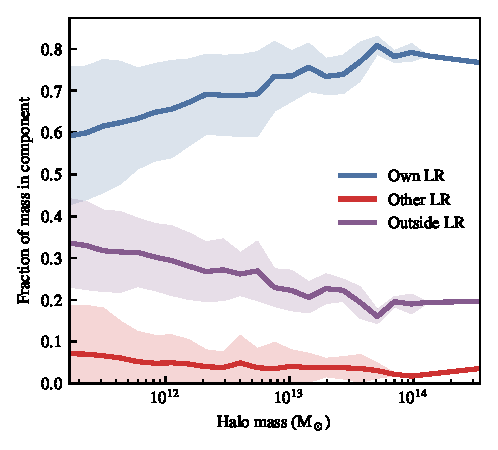
\includegraphics[width=\columnwidth]{generated_figures/component_fraction_vs_halo_mass_both.pdf}
	\caption{The fraction of total baryonic mass in a given halo at $z=0$
	as a function of halo mass. These values are computed using the
	lagrangian region IDs that were assigned to the gas and star particles
	in the initial conditions. See Figure \ref{fig:splitmassfrac} for a
	breakdown into stellar and gaseous components. The shaded regions show
	a single standard deviation of variance in the mass fraction for that
	bin, and do not include errors from halo sampling bias or cosmic
	variabnce. \blue{Might be worth including those errors in our analysis?
	I presume this is why our errors drop off as a function of halo mass,
	rather than this actually being an effect of the scatter getting
	lower.}} \label{fig:massfrac} \end{figure}

Once this analysis has been performed it is possible to see the fraction of
baryonic mass at $z=0$ that originates from the lagrangian region of a given
halo (see Figure \ref{fig:massfrac}). There is a significant difference in the
contributions from the gaseous and stellar components to this mass fraction;
see Figure \ref{fig:splitmassfrac}. This data is for every halo in the box, and
hence does not include any cuts based on the particlar neighbourhood of these
halos; a significant fraction of the scatter here is likely to come from
isolated halos, versus those in clusters and other noisier environments. This
analyis shows that a significant portion (up to 20\%) of the stellar mass of a
Milky-Way mass halo may come from the lagrangian region as defined by a
\emph{different halo}.

\blue{It would be nice at some point to include isolation criteria here. After
speaking to some people who do zoom-ins of clusters, it seems that they
actually only generate hydrodynamics particles that are within the LR (as
defined by the dark matter out to ~3 Mpc of the halo of interest). If we see
significant transfer even for isolated, milky way mass, galaxies, that would
really break things like APOSTLE. Thankfully at the moment they have chosen
very isolated halos, though.}

\begin{figure*} \centering
	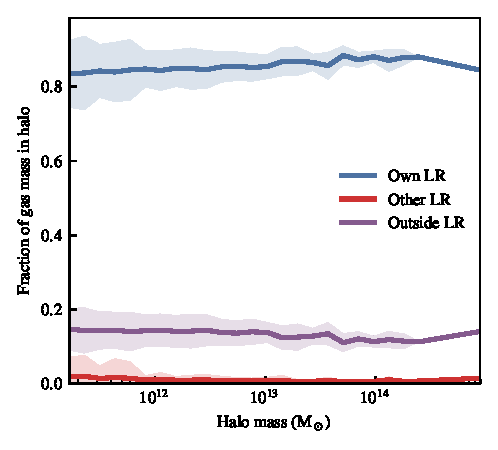
\includegraphics[width=0.495\textwidth]{generated_figures/component_fraction_vs_halo_mass_gas.pdf}
	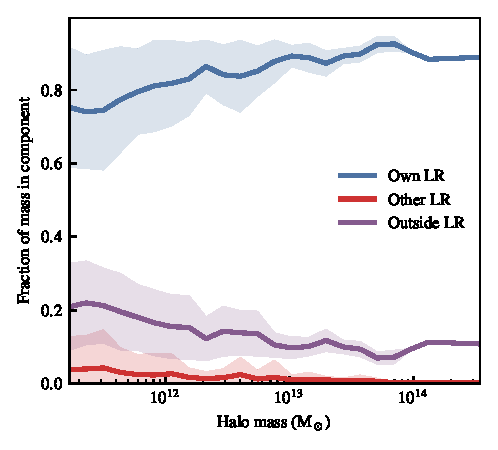
\includegraphics[width=0.495\textwidth]{generated_figures/component_fraction_vs_halo_mass_stellar.pdf}
	\caption{Left: fraction of gaseous mass at $z=0$ in each halo from each
	component; right: fraction of stellar mass at $z=0$ from each
	component. Note that there is significantly more transfer shown in the
	gaseous component. Gas that is transferred between lagrangian regions
	must be given time to cool before being able to form stars. As the
	events that enable transfer are typically very energetic (AGN, stellar
	feedback, accretion), it is unlikely that the cooling time will be
	short enough to form stars by the end of the simulation for most
	transfer.} \label{fig:splitmassfrac} \end{figure*}

\subsection{Redshift Evolution}

\blue{We should re-run the above analysis at a lower redshift, just to check
that the transfer is actually lower, like we already had before the disaster.}

\subsection{Radial Trends}

\begin{figure} \centering
	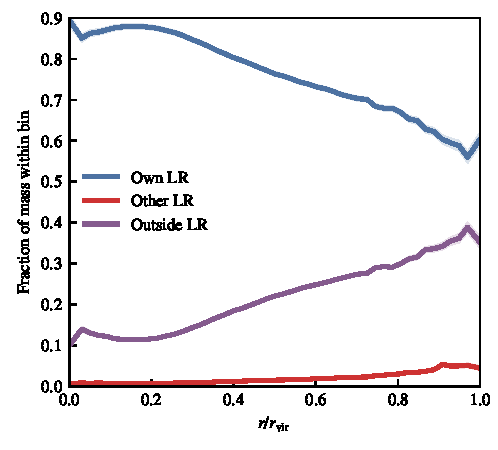
\includegraphics[width=\columnwidth]{generated_figures/radial_distance_plot.pdf}
	\caption{The dependence of mass fraction split by component as a
	function of radius, normalised by the virial radius for each halo.
	Every halo with $10^{12} \leq $ M$_{\rm halo}$ $ < 10^{13}$ M$_\odot$
	is stacked in this plot, with the shaded regions giving standard errors
	around the mean. Solid lines show the trends for gas, with the dashed
	lines showing the same but for the stellar component of the halo. 50
	bins were spaced linearly in radius.} \label{fig:radialmassfrac}
\end{figure}

The mass fractions contributed from various components to each halo appear to
be relatively independent of halo mass (see Figure \ref{fig:massfrac}), however
this may not be true within each individual halo. In Figure
\ref{fig:radialmassfrac} the mass fraction contributed to the halo is shown as
a function of radius. As expected, more gas in the center of the halo comes
from the corresponding lagrangian region, but interestingly this only
approaches ~60\%, suggesting significant transfer \emph{into halos} still takes
place for gas that ends up at the bottom of the potential well at $z=0$.

Also note how the mass fraction of stars from the own lagrangian region of the
halo drops as a function of radius. This suggests that a large number (~30\%)
of these stars were formed ex-situ. \blue{Perhaps this is a good place to
reference other work... This is a surprisingly high number}. Note, again, that
around ~15\% of the stars at the center of these halos are formed from gas that
was not present in the initial lagrangian region of this halo. This is
surprising, as this transfer must have taken place relatively early to ensure
that the gas was able to cool and form stars.

\section{Halo-indepdent measures of baryonic flows}
\label{sec:haloindependent}

\begin{figure*} \centering
	\includegraphics[width=\textwidth]{figures/kspafig.pdf} \caption{A
	diagrammatic representation of the distance measure. On the left, the
	initial conditions are shown. The blue dark matter particles each find
	their closest dark matter and gas (red) neighbour. These particles are
    then tracked to the final state of the simulation at z=0 (right) and the
    distance between them calculated again to assess the relative motion of dark
    matter and baryons.} \label{fig:distancemeasure}
\end{figure*}

\subsection{Using inter-particle distances to describe transfer}

Usually, analysing how baryonic and dark matter move differently requires the
use of a halo finder, to identify structures between which gas can flow.
However, if the gas and dark matter become decoupled, it should be possible to
see this effect without having to consider bound structures at all.

To find how separated the dark matter becomes from the gas, two distances
\emph{in the final snapshot at $z=0$} are considered. First, the distance
from each dark matter particle to the corresponding closest dark matter
neighbour in the \emph{initial conditions}, i.e. the distance
\begin{equation}
    r_{ij, ~z=0} = \sqrt{ \left| \mathbf{x}_{i,
    ~z=0} - \mathbf{x}_{j \ni \min(r_{ij, ~z=z_{ini}}), ~z=0} \right|^2 }
    \label{eqn:minimal}
\end{equation}
where $\mathbf{x}_i$ is the position of particle $i$, and $\mathbf{x}_i -
\mathbf{x}_j$ is wrapped within the periodic box. The corresponding distance
between the dark matter particle and the closest gas neighbour in the initial
conditions is also considered, $r_{\rm gas}$. A diagrammatic representation of
this is given in Figure \ref{fig:distancemeasure}. Star particles at $z=0$ are
ID matched with their gas progenitors, where at all possible. 

\subsection{Distribution of Distances}

\begin{figure} \centering
	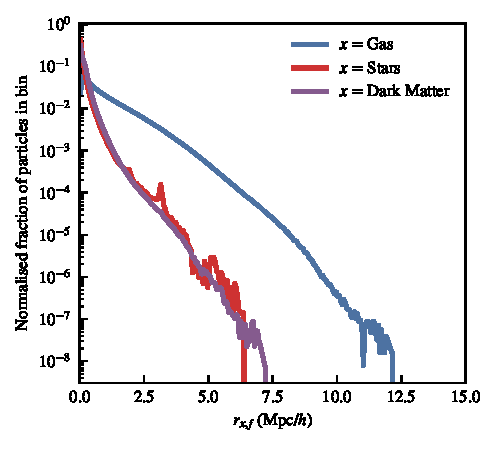
\includegraphics[width=\columnwidth]{generated_figures/neighbour_analysis_simple_histogram.pdf}
	\caption{The distribution of all distances to particles at $z=0$. Note
	the similarity between the dark matter distribution and the stellar
	distribution, and how different they are to the gas with the associated
	long tail.} \label{fig:alldistances}
\end{figure}

Now that the distances at $z=0$ have been identified it is possible to
compare how mixed the dark matter has become, compared to the gas, beginning
with the distribution of final particle distances from their initial
neighbour. In Figure \ref{fig:alldistances} the similar dynamical
distributions of the stellar and dark matter components are shown, with the
gaseous component having a significantly longer tail. By the end of the
simulation, gas particles can end up around $15\hmpc{}$ away from their original
nearest neighbour; this can only occur due to the strong wind velocities that
are powered by the AGN in the simulation.

Such a large separation is certainly possible over the course of the
simulation in the \simba{} model. AGN winds are powered at around $10^4
\kms{}$, meaning that over the whole run-time of the simulation the maximal
distance that a wind can travel is nearly 150 Mpc; enough to wrap the whole
box three times. This is, however, clearly an extreme upper limit, with the
AGN winds being slowed immediately by interaction with the potential well of
the halo.

The similarity between the dark matter and stellar distribution is clear
here. Both follow extremely similar power-laws, something that must be
investigated further in the future. That the stars must form out of particles
that were initially gas in the simulation is nontrivial. The similar
distribution could simply owe to the dynamics of the gas that eventually
forms stars being dominated by gravitational forces, or the mixing timescale
being short enough that the majority of the stars become well mixed with the
dark matter by the end of the simulation. This could also possibly be a
signature of the gravitational softening, or be a signature of tidal
stripping of satellite halos, now thought to be a significant effect, as was
shown by \citet{vandenbosch2018}.

\subsection{Particle-by-particle comparison to dark matter}

\begin{figure} \centering
	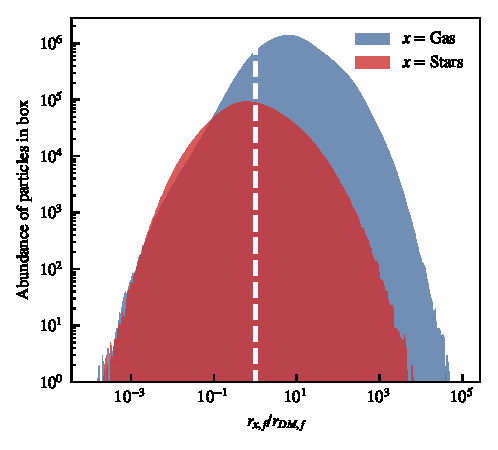
\includegraphics[width=\columnwidth]{generated_figures/neighbour_analysis_ratio_histogram.pdf}
	\caption{The distribution of relative final state distances for each
	dark matter particle to the appropriate gas and stellar (these
	correspond to $i$ in the bottom label) particles at $z=0$ normalised by
	the distance to the dark matter particle that was closest in the
	initial conditions. Note the significantly different distributions for
	gas and stars.}
\label{fig:dmvsstarvsgas} \end{figure}

Comparing solely the distributions of each particle type prevents the use of
the fine-grained particle data that is available. It is possible to compare,
for a given dark matter particle in the initial conditions, how much the
nearest baryonic particle has moved, compared to the nearest dark matter
particle. For each particle, the distance that the nearest dark matter
neighbour has travelled, compared to the nearest baryonic neighbour, is plotted in
Figure \ref{fig:dmvsstarvsgas}. The stellar distribution is highly symmetric
and peaks around $r_{\rm star}/r_{\rm DM} = 1$, implying that the stellar and
dark matter components have a very similar dynamical distribution (see also
Figure \ref{fig:alldistances}) but that this is not a \emph{local} effect.
The gas and dark matter do not become separated from the gas, as implied by the
original histogram, causing this effect; the stellar and dark matter are both
mixed in a similar way by the gravitational dynamics, completely randomly. If
there was a local effect here, we would see that the ratio of
$r_{\rm star}/r_{\rm DM}$ would be much more tightly constrained.

The same distribution for the gas, however, has a different signature.
$r_{\rm gas}/r_{\rm DM}$ peaks around 10, not 1, showing that gas ends up
preferentially further away than the neighbouring dark matter particle. That
gas behaves differently to dark matter is unsurprising; gas particles feel
repulsive forces from hydrodynamics, can be heated, and even get blown out of
galaxies. The strength of this effect, to blow gas out to distances of around
$\sim15 \hmpc{}$, corresponds approximately to the size of superbubbles in the
IGM created by AGN, suggesting that this is a signature of feedback
\citep{dave2018}. The effect of the gravitational dynamics can not be
decoupled from this result; the 9 orders of magnitude wide distribution is
also affected by mixing in the dark matter. The specific details of the
dynamics that causes this spread is still not understood, and must be
investigated in further work.

\section{Combining metrics}

\blue{In this section I would like to combine the two metrics and look at where the large-distance stuff comes from. We know that the majority of it ends up outside halos.}

\blue{I also think it's worth interrogating more the super large distances that stuff gets out to with the gas and dark matter. Where does that stuff live?}

\blue{Would be nice to have some visualisations here showing where the stuff comes from/ends up.}

\blue{I am guessing a lot of that gas will end up in the CGM. It would be nice to have a plot of chance of being from transfer v.s. position in halo.}

\section{Conclusions}
\label{sec:conclusions}


\section{Software Availability}

The software used in this paper for the Lagrangian transfer
calculations is available on GitHub\footnote{\url{https://github.com/jborrow/lagrangian-transfer}}. This paper is also available on
GitHub, along with data used to produce the majority of
the figures\footnote{\url{https://github.com/JBorrow/lagrangian-transfer-paper}}.

\end{document}
